% use paper, or submit
% use 10pt, 11pt or 12pt
% nopagenum removes the page numbers (final conference PDF paper)

%\documentclass[preprint, paper,11pt]{AAS}	% for preprint proceedings
\documentclass[paper,11pt]{AAS}		% for final proceedings (20-page limit)
%\documentclass[paper,12pt]{AAS}		% for final proceedings (20-page limit)
%\documentclass[paper,10pt]{AAS}		% for final proceedings (20-page limit)
%\documentclass[cover, article,11pt]{AAS}		% for journal paper version
%\documentclass[submit]{AAS}					% to submit to JAS

\usepackage{bm}
\usepackage{amsmath}
\usepackage{subfigure}
%\usepackage[notref,notcite]{showkeys}  % use this to temporarily show labels
\usepackage[colorlinks=true, pdfstartview=FitV, linkcolor= black, citecolor= black, urlcolor= black]{hyperref}
\usepackage{overcite}


\usepackage{color}
\usepackage[normalem]{ulem} % added this to enable sout for strike outs



\definecolor{RED}{rgb}{1,0,0} 
\definecolor{BLUE}{rgb}{0,0,1} 
\definecolor{GREEN}{rgb}{0,0,1} 
\newcommand{\EditHPS}[1]{{\color{red} #1}}
\newcommand{\EditHPSd}[1]{{\color{red} \sout{ #1}}}
\newcommand{\EditEH}[1]{{\color{blue} #1}}
\newcommand{\EditEHd}[1]{{\color{blue} \sout{ #1}}}


\PaperNumber{18-XXX}
\CoverFigure{Figures/test} % Optional:  provide the path to the cover figure
\Conference{AAS Guidance, Navigation and Control Conference}
\ConferenceLocation{Breckenridge, Colorado}
\ConferenceDate{August 18--21, 2008}
% The following macros are used for the simulated journal article mode
\JournalName{Journal of the Astronautical Sciences}
\JournalIssue{Vol.~XX, No.~XX, XX--XX, XXXX, Pages XXX-XXX}
\JournalAuthors{Schaub}		% simulated article, authors in header
\JournalTitle{abcd}			% simulated article, brief title in header



\begin{document}


\title{Reinforcement Learning Techniques for Autonomous Aerobraking}

\author{Andrew Harris\thanks{Research Assistant, Ann and H.J. Smead Department of Aerospace Engineering Sciences, Graduate 
Student, University of Colorado Boulder, Boulder,
		CO, 80309 USA.},
		Hanspeter Schaub\thanks{Glenn L. Murphy Professor of Engineering, Department of Aerospace Engineering Sciences, 
			University of Colorado, 431 UCB, Colorado Center for Astrodynamics Research, Boulder, CO 80309-0431,  
		\href{mailto:hanspeter.schaub@colorado.edu}{hanspeter.schaub@colorado.edu}}
}


\maketitle{} 		


\begin{abstract}
This work outlines a preliminary scheme for the development of autonomous aerobraking decision-making from a probabilistic 
perspective by formulating the problem using Partially-Observable Markov Decision Processes (POMDPs) solved using reinforcement 
learning techniques. Aerobraking operations about planets with atmospheres provides a promising means for 
improving the performance of interplanetary missions, but uncertainties in the modeling of planetary atmospheres necessitate 
large operations teams which raise mission cost and risk. This paper reformulates the aerobraking problem in a discrete manner 
that enables the development of autonomous controllers capable of dealing with unmodeled atmospheric disturbances. A sample 
case based on the aerobraking campaign of the Mars Reconaissance Orbiter (MRO) is presented, demonstrating the performance of 
this approach versus a simple decision-making model. 
\end{abstract}


\section{Introduction}
Aerobraking, the use of drag forces about planetary atmospheres to reduce spacecraft velocities, has been proposed as a 
low-fuel method for controlling spacecraft since the dawn of the space age \cite{Vallado2013}. While it has achieved 
notable success in missions like the Mars Reconnaissance Orbiter and Mars Odyssey \cite{Long2008}, both missions suffered from 
long periods of sustained, high-tempo operations during the aerobraking maneuvers. These periods of sustained operations added 
dramatic overhead to the mission's cost and raised the grim spectre of human error. Due to these costs, NASA has made the 
development of on-board, autonomous aerobraking routines a priority \cite{Long2008}. Considerable efforts in this realm have 
already 
been undertaken, focusing on the development of routines to estimate spacecraft orbits and periapsis parameters on board. 
Typically, autonomous aerobraking is considered to consist of two major steps: the evaluation of the current spacecraft orbit 
(autonomous orbit determination),
and 
related parameters, and the selection of maneuvers to ensure that the spacecraft safely moves towards its desired orbit (c.f. 
Figure \ref{fig:aerobrakingChoices}). This work aims to address the later problem.

\begin{figure}[!b]
	\centering
	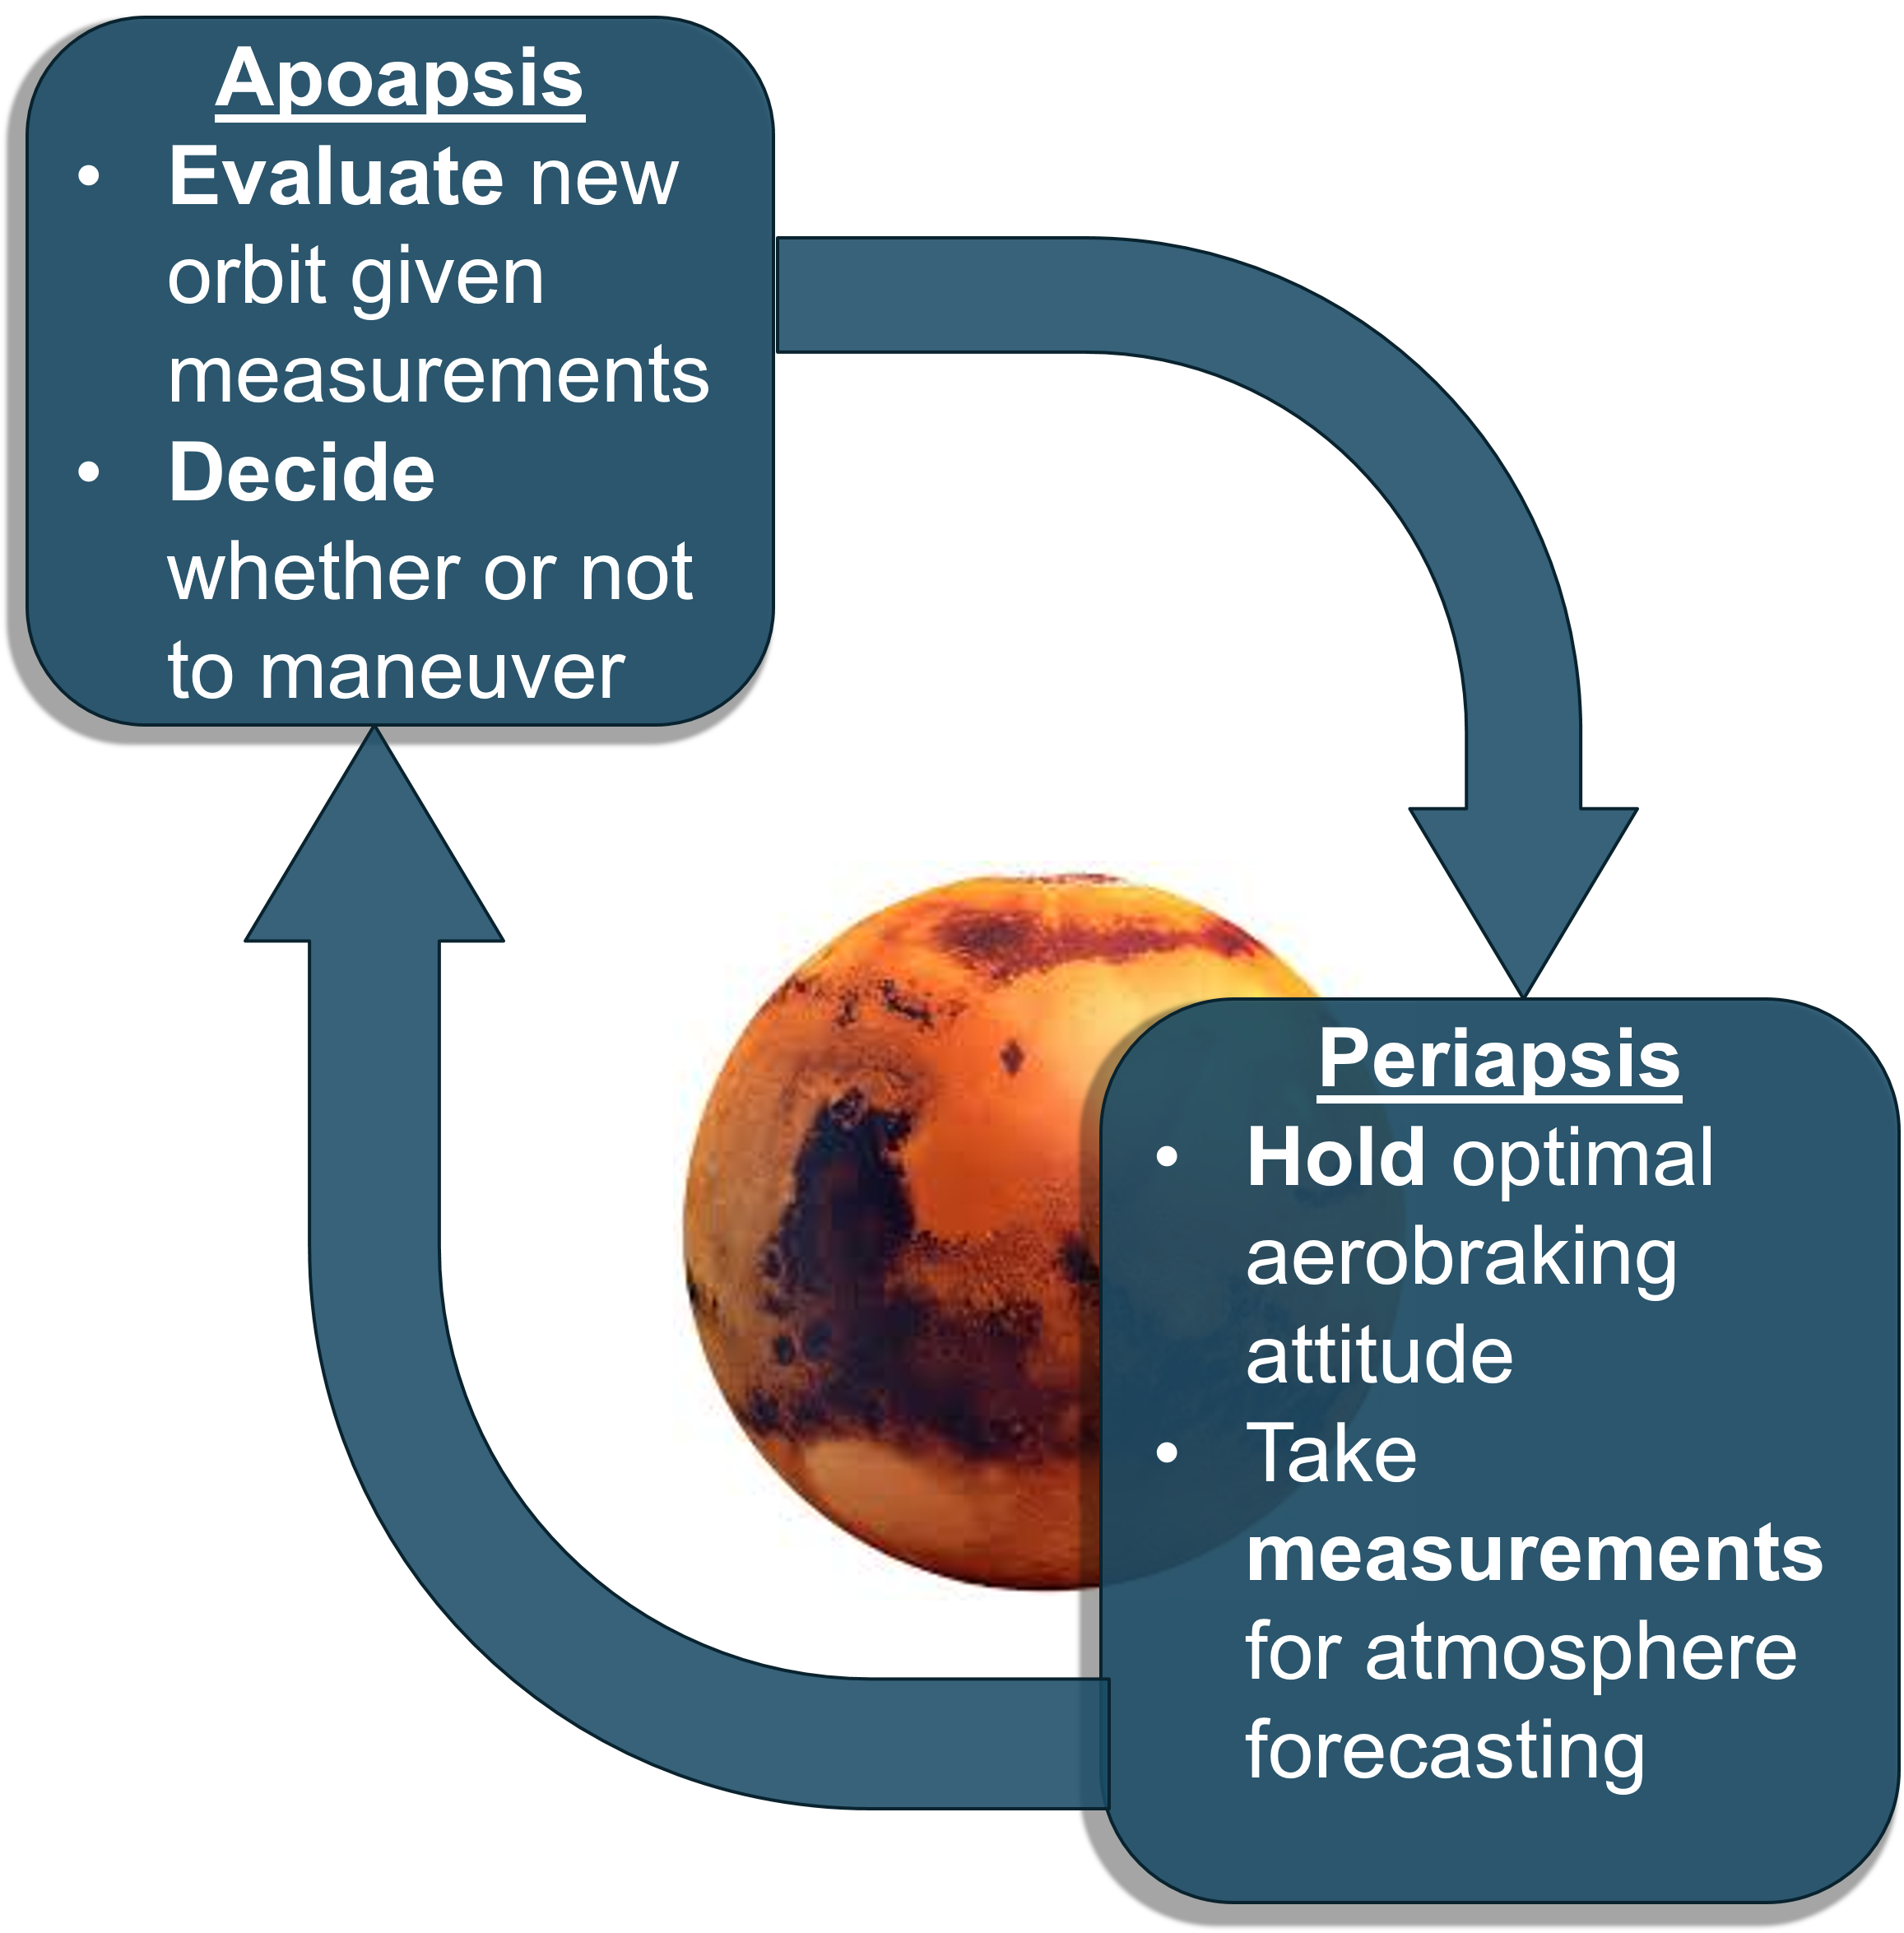
\includegraphics[width=2.5in]{aeroDecisionmaking.png}
	\caption{Graphical depiction of autonomous aerobraking phases, issues.}
	\label{fig:aerobrakingChoices}
\end{figure}

Spacecraft undergoing aerobraking have a number of constraints. First and foremost, aerobraking is undertaken to enter a 
desired orbit, typically by reducing an initial orbital semi-major axis. Additionally, spacecraft are typically only built to 
withstand certain levels of aerodynamic forces, including thermal effects from compressive heating. These forces, combined with 
a model of the atmosphere, are used to drive acceptable aerobraking trajectories (referred to as ``corridors.'') Over a given 
pass, orbital energy is dissipated due to drag forces; while this most directly reduces the radius of apoapsis as a burn at 
periapsis would, the length of a given pass also causes the radius of periapsis itself to decrease. Under an exponential 
atmospheric model, this consistent small decrease in the radius of periapsis can lead to  exponentially growing drag forces, 
eventually resulting in a catastrophic collision with the planet. To prevent this, spacecraft must fine-tune their orbits prior 
to 
an atmospheric pass to prevent re-entry and excessive aerodynamic forces while still ensuring that the spacecraft moves towards 
its desired orbit.

This process is complicated by the mercurial, difficult-to-model nature of planetary atmospheres. While atmospheric modeling 
has produced qualitative advances in our understanding of how atmospheres behave, prediction of atmospheric densities remains a 
challenge, and uncertainty in atmospheric density predictions drives uncertainty in spacecraft trajectory propagation. As such, 
any on-board aerobraking algorithm must be able to compensate for uncertainty in its prediction of atmospheric parameters. 
By nature, the atmospheric density is difficult to directly observe and is frequently inferred from measurements of drag forces 
acting on spacecraft \cite{Sutton2008}. 

Partially-Observable Markov Decision Processes (POMDPs) are a general class of problems in which observable and unobservable 
states operate as Markov processes affected by selected decisions. Additionally, rewards are provided based on combinations of 
actions of system states; typically, the objective of a given POMDP problem is to select decisions such that the overall reward 
is maximized, opening the door to a variety of solution methods \cite{Sutton2012}. 

POMDPs are classically described in discrete space and discrete time. A given system's state is captured within this framework 
as $s \in S$, possible actions are captured as $a \in A$, and unobservable variables are captured as $z \in Z$. The transitions 
from a given state $a_k$ to the next state $a_{k+1}$ is given by the conditional probability $P(a_{k+1}|a_k, z_k, d_k)$. A 
typical elemental POMDP can be seen in Figure \ref{fig:classicalPOMDP}. 

This work aims to reformulate the aerobraking problem as a POMDP and apply conventional POMDP solutions, such as Value 
Iteration, to produce an ``optimal'' policy under aerodynamic constraints. This solution will be compared to simple a-priori 
decision-making rules to demonstrate the flexibility of the outlined method in response to system uncertainty without human 
feedback in the loop.

\begin{figure}[!b]
	\centering
	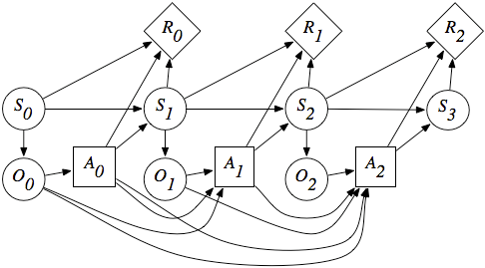
\includegraphics[width=2.5in]{classicalPOMDP.png}
	\caption{Classic Baysian network POMDP with states $s_i$, actions $A$, and rewards $R$. }
	\label{fig:classicalPOMDP}
\end{figure}

\section{Nonlinear System Definition}
\subsection{Continuous Time, Continuous State-Space, Continuous Action-Space Definition}

Generally, the orbit of a spacecraft about a massive body is governed by a second-order nonlinear ordinary differential 
equation, displayed in Equation \ref{eqn:gravEqn} \cite{Vallado2013}. 

\begin{equation}
\ddot{\mathbf{v}} = \frac{\mu}{r^3} \mathbf{r} + \mathbf{a}_{\text{perturb}}
\label{eqn:gravEqn}
\end{equation}

To account for the presence of atmospheric drag, we can compute the time-dependent drag acceleration $a_D$ by applying Equation 
\ref{eqn:dragEqn} \cite{Vallado2013} using the known ballistic coefficient for the spacecraft, the spacecraft's velocity 
relative to the planet's atmosphere, and the local neutral atmospheric density $\rho$. The local density is assumed to be given 
by a simple exponential density model of the form shown in \ref{eqn:expAtmo}. Note that because the drag force only acts in 
opposition to the spacecraft's velocity, it can only affect the shape and size of the planar components of the spacecraft's 
orbit; no inclination-changing maneuvers are possible under this simple drag model \cite{Sutton2008}.

\begin{equation}
\mathbf{a_D} = -\frac{1}{2} C_{B} \rho v^2 \hat{\mathbf{v}}
\label{eqn:dragEqn}
\end{equation}

Uncertainty in the atmospheric neutral density $\rho$ over an aerobraking is a 
primary driver of aerobraking risk. While a number of highly complex atmospheric models exist for the planets, we simplify the 
problem by selecting a two-parameter exponential atmospheric model of the form given by Equation \ref{eqn:expAtmo}. 

\begin{equation}
\rho = \rho_0 e^{\frac{-h}{h_0}}
\label{eqn:expAtmo}
\end{equation}

From this setup, we see that our full problem consists of six spacecraft states given by the position and velocity vectors $r$ 
and $v$ and two unobserved variables $\rho_0$ and $h_0$. 

We assume here that other perturbations, such as higher-order gravity terms, solar radiation pressure, electromagnetic forces, 
and 3rd-body effects, are small over the timespan considered and given our orbital geometry. In practice, this assumption will 
likely present an issue for effective planning, as they can dramatically alter the trajectory of a given spacecraft.

With the underlying dynamics established, we seek to define ``goals'' for the optimal decision-making strategy in continuous 
space. We will restrict ourselves to selecting an orbit of the form $\{r_a x r_p\}$, where $r_a$ and $r_p$ are the altitudes 
of apoapsis and periapsis respectively; this is a common shorthand for writing a given orbit (for example, the ISS is in a 
$400\text{km} \times 450\text{km}$ orbit about the Earth \cite{Vallado2013}.)

\section{Discretization Approach}
While continuous POMDP solvers exist, this work aims to first address the aerobraking problem by approximating it as a 
discrete-time, discrete-state stochastic process. The discretization of the continuous system outlined in the previous section 
is outlined here.

 First, the decision process is restricted to occur only at apoapsis, allowing us to consider the ``discrete'' transition of 
 the radii 
of apoapsis and periapsis over each orbit. This approach is sensible due to the underlying 
nature of the control problem; burns to affect periapsis are most efficient when conducted at apoapsis. Applying this approach 
leads to a discrete-time system in orbits. An important caveat is that each time-step is not actually of constant length, as 
the period of an orbit is governed by its semi-major axis. However, this is a reasonable approximation under the assumption 
that the orbit is well-determined 
through optical navigation or other means.

In general, the variables $\rho_0$ and $h_0$, the surface density and scale height respectively, vary with time, solar flux, 
geomagnetic variation, and other complex phenomena. While complex, high-fidelity models of atmospheric variation are publically 
available, this initial analysis assumes that $\rho_0$ and $h_0$ are normally distributed about their reference values and 
remain constant over each atmospheric pass.

A major issue with discretization is the orbit of the spacecraft itself, which is typically represented in six dimensions as 
either a set of orbital elements or as the spacecraft's six-dimensional position and velocity, both of which evolve in 
continuous space. While continuous-space methods for approximately solving POMDPs exist, preliminary work in this area has 
instead taken the 
approach of reducing the six-dimensional, continuous representation of the spacecraft's orbit to a two-state, discrete 
representation. 

Our assumption that aerodynamic forces act only within the spacecraft's orbital plane implies that aerobraking can only be used 
to affect the spacecraft's semi-major axis and eccentricity. These variables directly drive the spacecraft's orbital radius of 
periapsis and apoapsis. The radius of periapsis indirectly ties into the drag force experienced by governing the level of 
atmospheric density encountered by a spacecraft over a given pass, while the radius of apoapsis completes the knowledge of the 
spacecraft semi-major axis and eccentricity. For the purposes of this project, the spacecraft radii of apoapsis and periapsis 
were selected as the state variables to be controlled. In a similar manner, the space of ``actions'' taken by the spacecraft 
must be discretized.

To discretize these state variables, continuous-space states were sampled into a series of $n$ logarithmically-spaced bins 
ranging from the planet surface to the initial orbit altitude. The action space was discretized into three simple actions: 
doing nothing (Action 1), raising the continuous radius of periapsis by 5\% (Action 2), or lowering the continuous radius of 
periapsis by 5\% (Action 3). These broadly capture the affect 
of ``unit'' burns at periapsis. 

\section{Reinforcement Learning}

Modern machine learning techniques frequently use so-called ``reinforcement-learning'' approaches to address problems 
formulated as POMDPs. These techniques can design robust, flexible control schemes for  complex, non-linear, uncertain systems 
with relatively small design efforts. Additionally, they are readily extended to on-line techniques that can be used to 
incorporate real data

\subsection{Value Function Definition}
Critical to the function of any reinforcement learning technique is the definition of a so-called ``value function'' or 
inversely a ``cost function.'' As stated previously, the objective of any reinforcement learning algorithm is to maximize the 
``reward'' or ``earned-value'' over a specified time-span given a particular set of actions. If the reinforcement learning 
algorithm is effective and maximizes the earned value, the designer's problem is reduced to selecting an appropriate value 
function.

In the case of the aerobraking problem, several sources or sinks of value present themselves. Positive actions to consider for 
use in the value function include:
\begin{itemize}
	\item Achieving specified apoapsis/periapsis targets
\end{itemize}

Negative values to consider include:
\begin{itemize}
	\item Maneuvering
	\item High aerodynamic or thermal load
	\item Total aerobraking phase length
\end{itemize}

This space of design variables will be explored for a combination that produces successful aerobraking ``policies.'' 

\subsection{Tool Concept of Operations}

The validity and utility of this approach is predicated on two issues: whether it provides the same performance of 
``traditional'' rule-based aerobraking methods, and whether it can extend the state of the art by enabling spacecraft to 
``learn'' properties of the atmosphere used for aerobraking on-line. From this, the following concept-of-operations for such an 
approach is defined:

\begin{itemize}
	\item \textbf{Algorithm and Value Function Definition:} First, designers would select a suitable reinforcement learning 
	technique and value function to represent the desired ``success'' criterion.
	\item \textbf{Model Learning in Simulation:} Simulated data representing best-understood conditions of the aerobraking 
	environment would be used to train the aforementioned algorithm to achieve desired aerobraking performance.
	\item \textbf{Online Learning:} Once implemented ``on-line,'' the control algorithm would further update its atmospheric 
	model or policy in response to actual, non-simulated sensor readings. 
\end{itemize}

Unfortunately, the third step--on-line learning using real sensor data--is difficult to justify for research. For the purposes 
of this work, on-line learning performance will be tested using higher-fidelity models of the aerobraking problem. 

An important aspect of this research is the understanding of what is gained by including on-line learning during aerobraking. 



\section{Conclusion}

The aforementioned modeling and learning approach presents a credible method for improving the autonomy and performance of 
future aerobraking spacecraft. Comparisons between traditional rule-based aerobraking schemes, reinforcement-learned planning 
techniques using static training data, and techniques using on-line training methods will be compared on performance metrics 
like fuel use, aerobraking maneuver duration, and actual aerodynamic and thermal loads during aerobraking passes.

\bibliographystyle{AAS_publication}   % Number the references.
\bibliography{final.bib}   % Use references.bib to resolve the labels.


\end{document}
